\chapter{Implementation}
\label{chap:implementation}
When implementing a real time mesh deformation system certain choices must be made.
Firstly one must decide upon the model to use for the mesh deformation itself, i.e. are we algorithmically solving these problems using proper physics, or do we more brute force it through particle simulation. The algorithmic approach using proper physics will usually yield more realistic results, however, they are usually more complicated to implement,
and might not meet the performance requirements of games. The more brute force approaches such as spring-mass spring systems are usually easier to implement,
and gives good enough results.
Following the decision of models we need to decide on an integration scheme, how should we model the changes in acceleration, position, and velocity of our vertices?
Many different integration schemes exits, such as explicit Euler integration, Runge Kutta, or Verlet Intergration, all with different properties and difficulty of implementation.
Following these choices it is possible to start implementing a mesh deformation system.

\todo{Talk about how the deformation is done without mentioning springs first. I.e. you apply force to it.}
\todo{Also mention the importance of damping.}
\todo{Discuss semi-implicit euler integration scheme. Show math and implementation, discuss advantages and disadvantages with it.}
\todo{Motivate that you choose both your "physics model" and your integration scheme}

\section{What is Spring Mass Damping?}
The spring mass damping model is usually presented in a quite intuitive manner.
Each vertex within a mesh is considered a point with its own mass.
Between the vertices are springs which try to hold the whole mesh together.
When no forces are applied to the vertices within the model, the length of the springs are in their desired \rephrase{"resting" state.}
When a forces are applied to the vertices and they start moving, the springs holding the vertices together will become stretched
and will try to get back to their resting state.

\todo{Add image}

\section{What is Semi-Implicit Euler Integration?}
Semi-Implicit Euler integration is perhaps the integration scheme that is easiest to follow, and comes most natural to programmers when they implement
movement in a realtime system for the first time. It is also a scheme used within a lot of physics engines\cite{gafferongames_integration}.
In Semi-Implicit Euler integration we keep the total accumulated force, velocity and position of each game object.
Upon each timestepped update of the system we divide all the force that has been applied to an object by the mass of the object to get the acceleration of the object.
Multiplying this acceleration with the timestep yields the change in velocity of the object, which added on the previous velocity becomes the new velocity.
This new velocity is then multiplied with the timestep and added to the position, reflecting the change in position over time.
The code for this can be seen in listing~\ref{code:semi-implicit_euler}

\begin{figure}
\begin{lstlisting}[label={code:semi-implicit_euler},language=csharp,caption={Semi-Implicit Euler Integration}]
private void Timestep(float deltaTime, GameObject go)
{
    var acceleration = go.force / go.mass;
    go.velocity += acceleration * deltaTime;
    go.position += go.velocity * deltaTime;
}
\end{lstlisting}
\end{figure}

\subsection{Advantages \& Disadvantages}
The largest advantage of the Semi-Implicit Euler integration is its ease of implementation, as well as the generally low computational complexity.
However, it is not entirely stable, meaning that you can get into situations where your numbers start exploding.

\section{What is Verlet Integration?}
Verlet integration 
\subsection{Advantages}
\subsection{Disadvantages}

\section{Implicit Springs - Ball Deformation}
\todo{Add video}
\todo{Add how force is applied, showing the picture from the tutorial}
Jasper Flick\cite{catlike_mesh_deformation} shows an implementation \rephrase{without explicit springs}, following a semi-implicit euler integration scheme.
In this implementation we keep a copy of the initial vertex positions, as well as a collection of the modified vertices.
Additionally, we keep a collection of the velocity of each vertex, which we update each time force is added to a vertex.
The springs come into play when updating the positions of all the vertices based on their velocities.
Each spring within this system is the vector between the initial positions of the vertices in the mesh and their current positions, as seen in figure \ref{fig:catlike_mesh_deformation_springs}.
Upon update of the vertices the force of a spring is applied to the velocity of a vertex in the direction of the spring, moving the vertex back towards its initial position (see listing~\ref{code:catlike_mesh_deformation_update}).

\begin{figure}
%\centering
    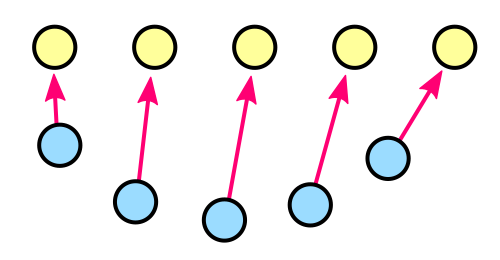
\includegraphics[width=\textwidth]{report/figures/catlike_mesh_deformation_springs.png}
    \caption{Modified vertices(yellow) are pulled towards their original position(blue) by the springs (pink)\cite{catlike_mesh_deformation}}
    \label{fig:catlike_mesh_deformation_springs}
\end{figure}

\begin{figure}
\begin{lstlisting}[label={code:catlike_mesh_deformation_update},language=csharp,caption={Catlike coding mesh deformation vertex update}]
private void UpdateVertex(int i)
{
    Vector3 velocity = mVertexVelocities[i];
    Vector3 spring = mDisplacedVertices[i] - mOriginalVertices[i];
    spring *= UniformScale;
    velocity -= spring * SpringForce * Time.deltaTime;
    velocity *= 1f - Damping * Time.deltaTime;
    mVertexVelocities[i] = velocity;
    mDisplacedVertices[i] += velocity * (Time.deltaTime / UniformScale);
}
\end{lstlisting}
\end{figure}

\subsection{Usage}
As seen from the video, although simple, the implementation provides quite a lot of flexibility, toying with the different variables
can lead to some interesting visual effects.
For example, applying negative force to the sphere can be used to create a visual effect similar to that of a star being swallowed by a black hole.
Applying outward force from the inside of the model can create a relatively convincing effect of something moving around inside the object.
Giving the sphere a high SpringForce will lead to it being harder to deform, and more bouncy when trying to return to its original shape.

\subsection{Limitations}
As previously mentioned the implementation is quite simple, but has some limitations.
As mentioned by Flick\cite{catlike_mesh_deformation} this implementation is not a physics simulation, while the mesh is deformed
the colliders and physical representation of the object stays the same.
Additionally, none of the vertices are connected to each other through springs, and therefore move completely independent from each other.
This means that if we were to for instance pin two of the vertices to their initial position, and then apply force to the mesh
none of the other vertices would respect that two of them was locked in place, leading to less than satisfying results.




\section{Explicit Springs - Cloth Simulation}
\todo{This is a kinematic system, not a dynamic one, so should rename all the springs reference to constraints?}
Cloth simulation is a place where the springs are more apparent than the previous implementation.
The implementation seen in Figure \ref{fig:my_cloth_implementation_springs} shows all the springs needed to create a believable cloth simulation.
The implementation is based on that of Jesper Mosegaard\cite{mosegaards_clothing_simulation}.
Unlike the previous implementation, the springs here are explicit and ensure that vertices are not handled in isolation but rather are affected by the other vertices in the system.
This gives greater control in that it allows you to apply force to a specific vertex and the whole system responds, rather than having to apply the force to all the vertices.

\think{Need to start to segue into the spring types}

\todo{Find the gamasutra article that discussed this}


\begin{figure}
%\centering
%    \caption{\todo{Insert figure}}
    \label{fig:my_cloth_implementation_springs}
\end{figure}


\subsection{Spring Types}
There are three types of springs within this implementation, all serving the same purpose of holding the model together,
but in different ways.

\subsubsection{Structural Springs}
The structural springs are the vertical and horizontal connections between the vertices,
ensure that the model stays in one piece.
However, they alone are not enough, as the model can collapse into itself in a two dimensional space.
\todo{Add small figure showing the structural springs}
\todo{Add small figure showing the model collapsing into itself with just structural springs}

\subsubsection{Shear Springs}
Shear springs fixes the issue mentioned above by a connection between each vertex and their diagonal members.
When the vertices are about to start collapsing in on themselves the shear springs will push them apart again.
\todo{Rewrite this to make it clearer what I mean with 3 dimensional space}
These springs also helps the model to act in a three dimensional space.
Since the vertices no longer can collapse in on themselves they might need to make use of three dimensions to
resolve their collisions.
\todo{Add small figure showing the shear springs, and the model using shear springs}

\subsubsection{Bending Springs}
Technically you only need these two types of springs to create an ok looking cloth simulation,
however a third type of spring called bending springs can be added.
These are connected between each vertex and their second neighbour,
which can help fix cases where the second neighbour of a vertex is unrealistically placed in the system.
This in general leads to the cloth becoming more flat, as extreme differences between the vertices are corrected for
through the second neighbouring vertices.

\todo{Add Drawing}
% This might be what is creating wrinkles?
% Double check that this is actually the case.
% Without
%
% 1 -- 2
%      |
%      3
% With
% ------------|
% 1 -- 2 ---| |
%           3 -
\todo{Add small figure showing the bending springs, and the model using the bending springs}

\subsection{Implementation}
\todo{Go deeper into implementation, the meaning of the constants, showing the code, etc}

\subsection{Usage}
Due to its more sophisticated nature this implementation offers more flexibility than the previous one.
Simulation of entire pieces of clothes like curtains or flags are obvious ways of using this model.
However, it is not a requirement of the model that every vertex in a mesh are simulated and part of the mass spring system, you can also just simulate parts of it.
An example here is if you have a character wearing a dress, you probably do not need that every part of the dress
has realistic cloth physics, it is probably enough that just the bottom of the dress reacts to the environment
to create a believable appearance.
\todo{Add image showing parts of the model being simulated, as I don't think it is entirely clear from the text}

Another use case with this model could be to have cloth that tears at a certain point because it is stretched too much,
or that parts of the cloth is cut off. This should not be too difficult, you would need to remove the springs between
the vertices that have been disconnected from the rest of the model.
Additionally, you would have to ensure that all the cuts were in line with the triangles of the mesh.

\subsection{Issues}
Although there are many advantages of this model, like how it is relatively easy to implement, gives quite good results and cannot "explode", it does suffer from a few issues.
A problem with this implementation is that it can get into unsolvable states.
I.e. when you apply forces to model continously it can get into a situation where it never rests.
Such a situation can be seen in the following video \todo{Add video}.
Here the forces of gravity are continously being applied to the vertices, in the real world the bottom
of this cloth would stop moving after a while. However, in this implementation the cloth never stops moving
because the springs never manage to get into a situation where they all are "satisfied".
The number of times you need to iterate over the constraints to satisfy them is also an issue.
Too few iterations and the cloth will look too elastic, too many iterations and it can seem too hard,
additionally, the more iterations you add, the more processing time is needed, which can become a performance problem.

\subsection{Extensions}
Matthew Fisher\todo{Cite: https://graphics.stanford.edu/~mdfisher/cloth.html} suggests some extensions to the model,
such as quilting.
\todo{Expand on the points Matthew Fisher Brings up}

\todo{Bring up how this model can get into unsolvable states when forces are applied continously}
\todo{Having to iterate over all the springs multiple times isn't optimal}

\todo{Should I also look into the Catlike Coding water deformation thingy, as it is another way of doing mesh deformation}


\todo{The technology ahead, ask if this could be used with tesselation and be done on the GPU?}
\todo{Discuss how mass spring damper model also used for other stuff, such as water simulation. Look at Just Cause water implementation article on gamasutra}
